\clearpage

\section{DC component removal}

\begin{tcolorbox}	
	\begin{tabular}{p{2.75cm} p{0.2cm} p{10.5cm}} 	
		\textbf{Header File}   &:& dc\_component\_removal.h \\
		\textbf{Source File}   &:& dc\_component\_removal.cpp \\
        \textbf{Version}       &:& 20190225 (Daniel Pereira)\\
	\end{tabular}
\end{tcolorbox}

This block removes the DC/low frequency component of a complex time continuous signal.

\subsection*{Input Parameters}

This block has no input parameters.

\subsection*{Methods}

\bigbreak
DCComponentRemoval(initializer\_list$<$Signal *$>$ \&InputSig, initializer\_list$<$Signal *$>$ \&OutputSig) :Block(InputSig, OutputSig)\{\};
\bigbreak
void initialize(void);
\bigbreak
bool runBlock(void);

\subsection*{Functional description}

This DSP step removes the DC contribution on the input signal ,$S_\text{in}(t_n)$. This DC contribution can either be estimated by taking the average of the full input signal or from the average of a moving window. This contribution is then subtracted from the input
\begin{equation}
S_\text{out}(t_n)=S_\text{in}(t_n)-\text{mean}(S_\text{in}(t_n))
\end{equation}
\par
The effect of this DSP step is presented in Figure~\ref{fig:S4}. To better show the effect of this DSP, an exaggerated DC removal is presented in Figure~\ref{fig:S4EXAGERATED}, where it can be seen that the DC component is removed without introducing obvious discontinuities in the signal.
%
\begin{figure}[h]
\centering
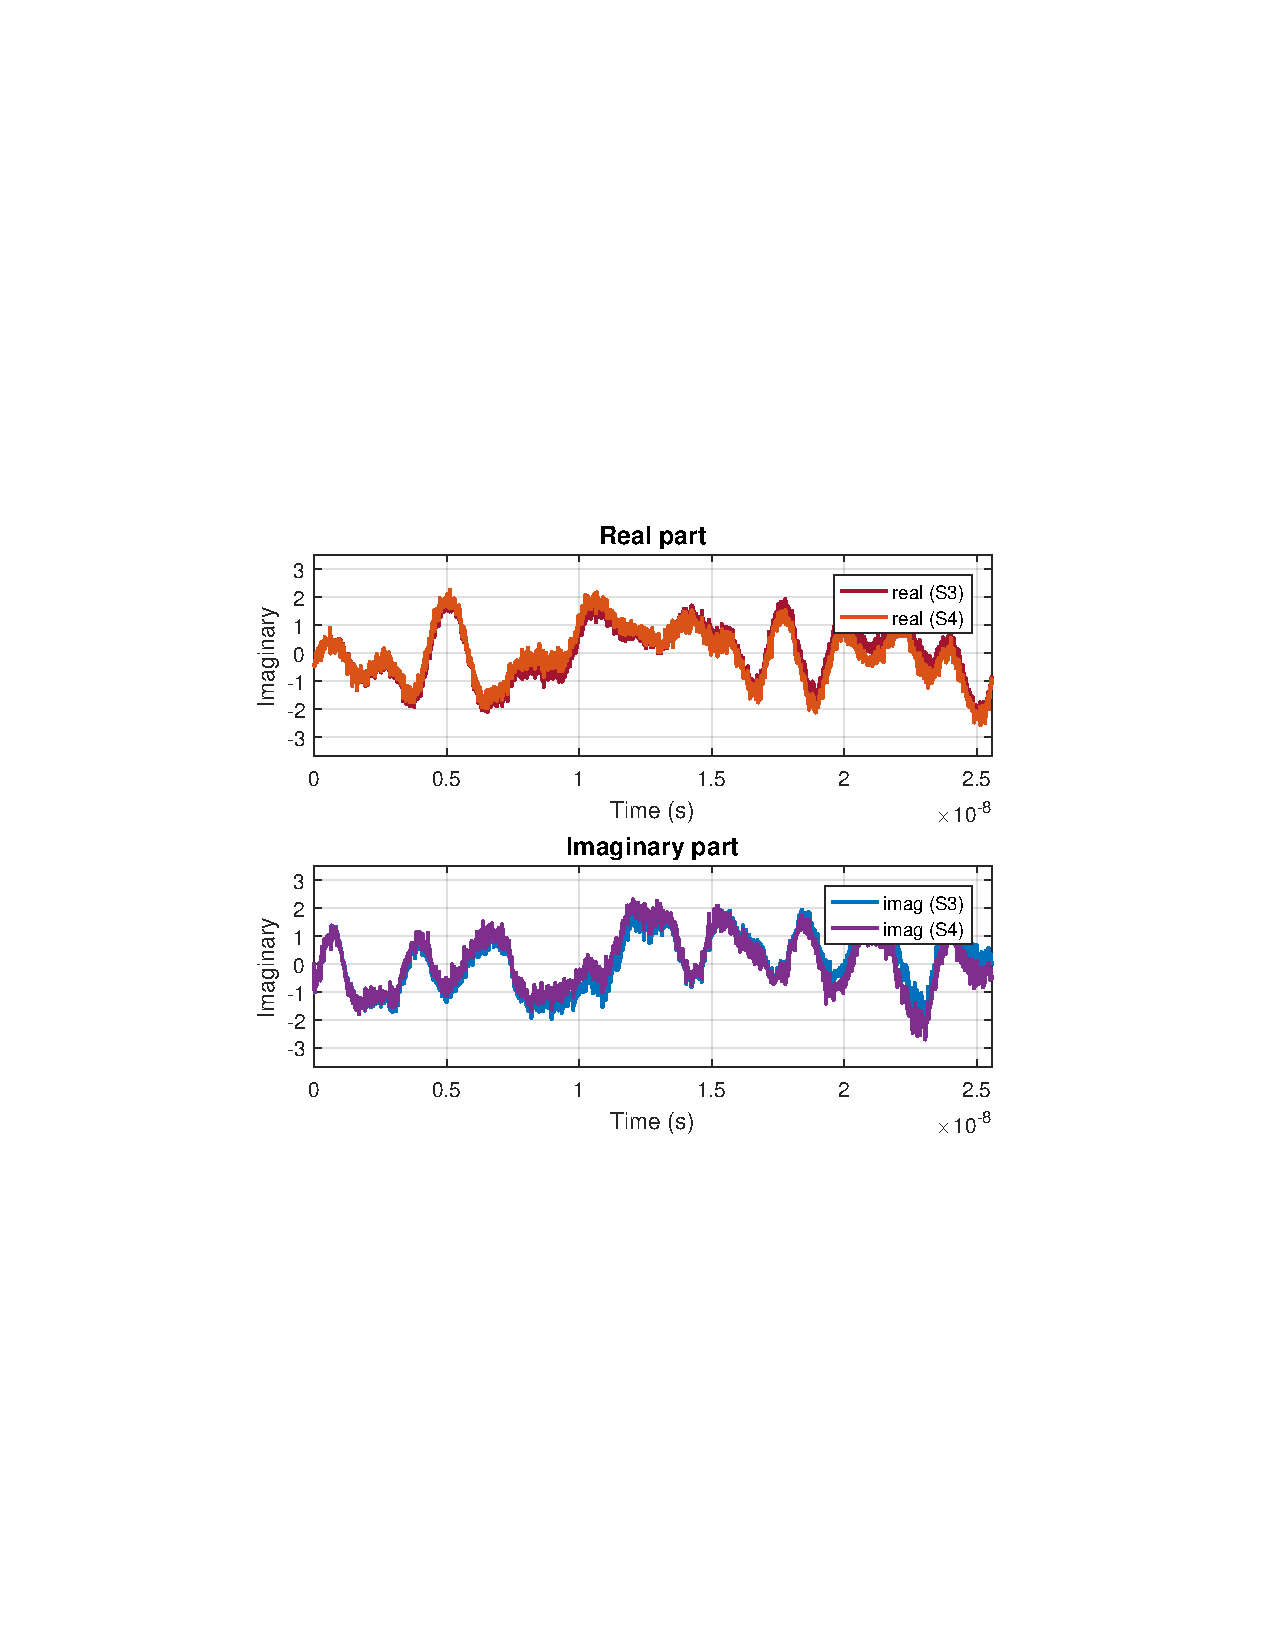
\includegraphics[trim={7cm 8cm 7cm 8cm},width=.3\linewidth]{./lib/dc_component_removal/figures/S4EXAGERATED}
\caption{Exaggerated DC component removal.}
\label{fig:S4EXAGERATED}
\end{figure}	
%
\subsection*{Input Signals}

\textbf{Number:} 1\\
\textbf{Type:} Complex signal

\subsection*{Output Signals}

\textbf{Number:} 1\\
\textbf{Type:} Complex signal

